\par{Kernel shown in \ref{more_work_kernel} its our attempt to give every \emph{work item} more computational load, that way decreasing the
    effects of scheduling and spawning overhead of \emph{work items} and \emph{work groups}.}
\par{...\ref{MoreWork}\ref{MoreWorkComp}}

\lstinputlisting[caption={Kernel with more work per \emph{work item}.}, label={more_work_kernel}, 
                style=customc]{/Users/clalanne/GitHubProjects/OpenCLNotes/src/code/more_work.c}

\begin{figure}[!h]
    \centering
    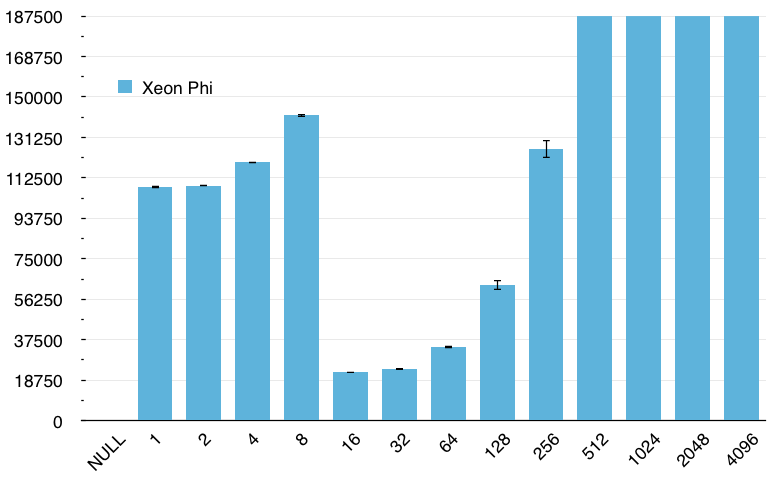
\includegraphics[width=0.49\textwidth]{figures/opt1_phi.png}
    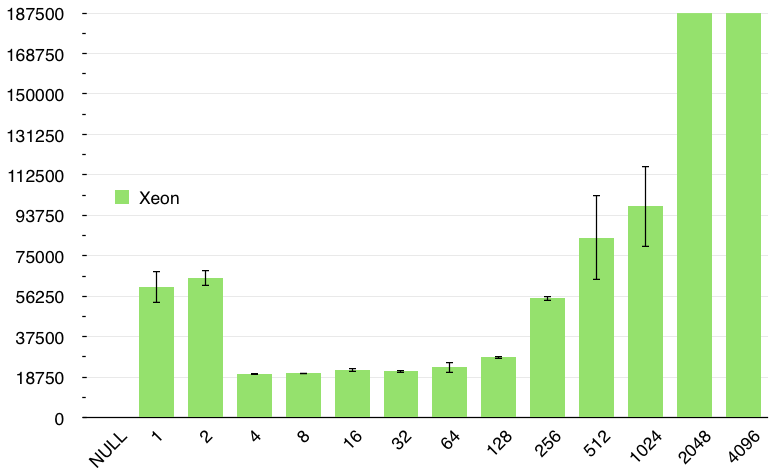
\includegraphics[width=0.49\textwidth]{figures/opt1_cpu.png}
    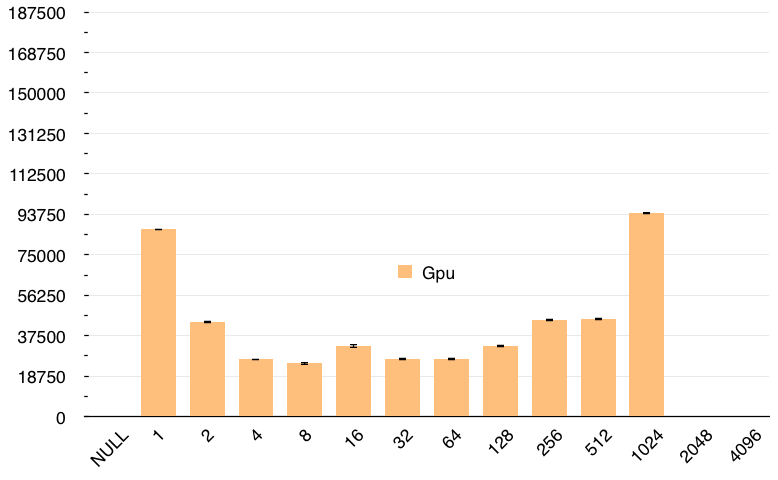
\includegraphics[width=0.49\textwidth]{figures/opt1_gpu.png}
    \caption{Matrix multiplication with more work in different architectures.}
    \label{MoreWork}
\end{figure}

\begin{figure}[!h]
    \centering
    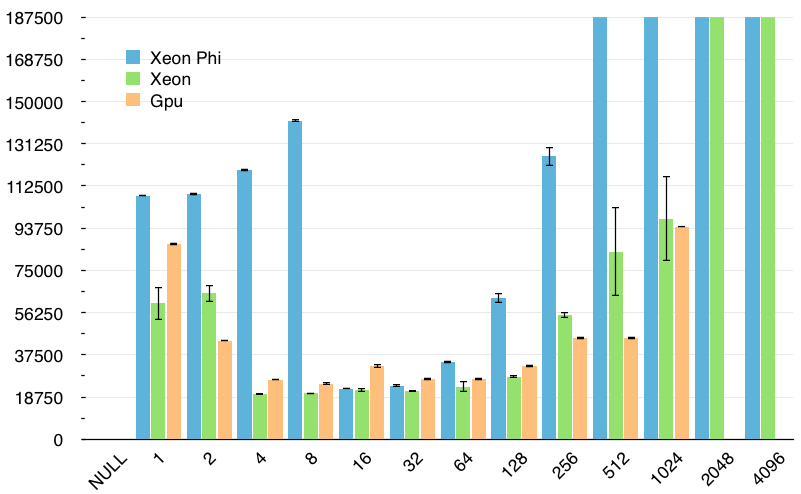
\includegraphics[width=0.6\textwidth]{figures/opt1_comp.png}
    \caption{Matrix multiplication with more work in different architectures comparison.}
    \label{MoreWorkComp}
\end{figure}

